\documentclass{beamer}
\author{Dilawar \\
  \texttt{dilawars@ncbs.res.in}
}
\title{Journal club talk}
\subtitle{On describing biological systems as computer programs}

\begin{document}
\maketitle 

\begin{frame}
  \frametitle{Languages in \textbf{Very Large Scale Integration}}
  \begin{itemize}
    \item Millions of components interacting in parallel. 
    \item Most of the computer
      programs execute sequentially (e.g. one line/fragment active at a time).
    \item Hardware description languages. All blocks are alive all the time,
      listening to each other.
    \item Model data as \textbf{ behaviour}.
  \end{itemize}
\end{frame}

\begin{frame}
  \frametitle{Contrasting biological systems}
  \begin{itemize}
    \item Cells are alive and their communication is distributed. Same in both!
    \item Cells multiply. Computer programs do not (sometimes they do).
    \item Two cells belonging to same class do not \textbf{behave} in the same
      way. Two components of circuit mostly do.
    \item Theory is not adequate, models are also only approximate.
  \end{itemize}
\end{frame}

\begin{frame}
  \frametitle{Frameworks for describing biological systems}
  \begin{itemize}
    \item Most of frameworks I read are proposed by computer scientists and are
      based on educated guess and \emph{feelings}. These people do not do
      modelling.
    \item Enough reasons to be skeptic.
     \end{itemize}
   \end{frame}

   \begin{frame}{Reactive systems}
     \begin{figure}
     \centering
     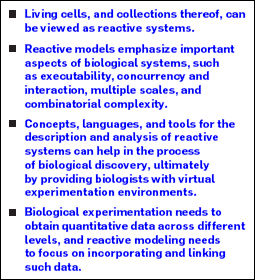
\includegraphics[width=0.6\textwidth]{./figures/bio_as_reactivity.png}
      \footnote{Biology as reactivity”, Jasmin Fisher, David Harel, Thomas A.
      Henzinger, ACM Comm, 2011.}
    \end{figure}
\end{frame}
    
\begin{frame}
 \frametitle{Abstract machines of biological system}
 \begin{figure}
    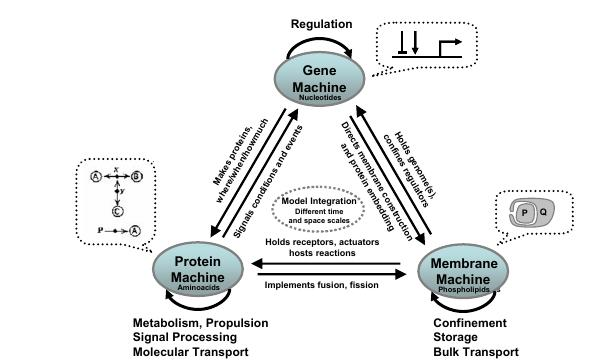
\includegraphics[width=\textwidth]{./figures/abs_machine.png}
    \footnote{Abstract machine of system biology, L. Cardelli}
  \end{figure}
\end{frame}

\begin{frame}
  \frametitle{Approach}
  \begin{itemize}

    \item Most of the frameworks suggested by Computer Scientists are based on
      “feelings”. That is not good enough.
    \item If I can scale, I will be \textbf{modular}.
    \item If I can easily optimize, I don't mind size of generated program.
    \item If I can parallelize, I will. 
    \item Talk to “bottom-up”/Modeling people. They should be able to integrate
      their “details” or models in the framework (with some work).
    \item Architecture: components should fit together. Inspirations from pipes : \texttt{ls -l | sort | head } 
  \end{itemize}
\end{frame}

\begin{frame}
\frametitle{A tool-maker point of view}
\begin{itemize}
  \item If I can't define/explain it, can I measure it (like electricity)?
  \item Not trying to explore Biology as such. Its a job for biologist.
  \item Aim is modest, give them a framework so Biologists can do it somewhat easily.
\end{itemize}

\begin{alertblock}{}
Complementary-MOS transistors have been modeled to very accurate details which
mimics their behavior. But its physics is yet to be understood satisfactorily.
\end{alertblock}
\end{frame}

\begin{frame}
  \frametitle{Challenges}
  \begin{itemize}
    

    \item Formal methods based on (model checking, Kripke Structures (Live
      Sequence Charts on steroids), Binary decision diagrams) at the topmost
      abstraction. Mature tools/libraries are available. 
    
    \item What is the meaning of “correctness” in Biological system? Does it
      exists?  How to model fitness, resilience, and robustness \footnote{
        Cerny, P., Henzinger, T.A. and Radhakrishna, A. Simulation distances. In
      Proc. Concurrency Theory 2010.}

    \item Theoretical challenge : horizontal linkage of heterogeneous
      components.  Experiences in VLSI can help a great deal in vertical linkage
      of abstractions. 
      

\end{itemize}
\end{frame}

\begin{frame}
\frametitle{Challenges}

Ability to integrate models. A common interface to fit any type of models
(C/Fortran/XML) (A lot of work) in a \textbf{reactive} framework.

  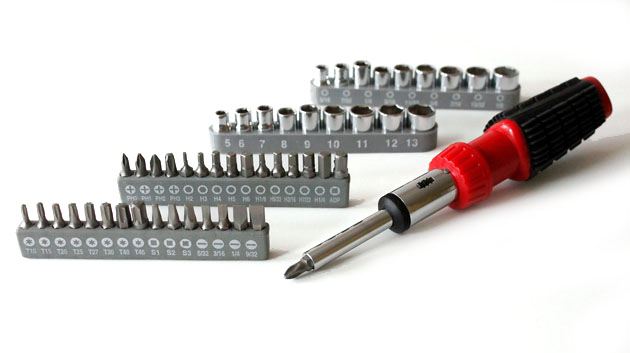
\includegraphics[width=0.8\textwidth]{./figures/multi-head-screwdriver.jpg}

\end{frame}

\begin{frame}
  \frametitle{Programmer's note}

  \begin{itemize}
    
    \item Various cell models approximate each others. \footnote{Upi suggested a
      paper, I don't remember it. There is an attempt here, \textit{A
    Complex-Valued Firing-Rate Model That Approximates the Dynamics of Spiking
Networks}, Evan S. Schaffer mail, Srdjan Ostojic, L. F. Abbotta, Oct 2013}. So
take one and extend it for development purpose.
    
    \item Partition the universe into smaller universes. Network flows,
      Gomory-Hu algorithms.
    \item Fast query databases, use them if available. Especially in the cache
      of processors.
    \item Locally synchronous, globally reactive.
A local synchronous unit has access to its sub-universe (put it in L3 cache,
rest goes into L2 cache).
    \item Projective geometry based architecture: symbol travels from  a node to
      any other node in at most 3 hops \footnote{Narendra Karmarkar}
  \end{itemize}
\end{frame}

\begin{frame}
  \frametitle{In the end $\ldots$}

  A good framework with an in-house language to describe and simulate Biological
  systems; or a thesis with title \textbf{How not to design a language for
  biology}.

\end{frame}

\end{document}

